% Chapter 4

\chapter{Apprentissage} % 4th chapter title

\label{Chapter4} % For referencing the chapter elsewhere, use \ref{Chapter4} 

L'objectif de cette section est de reconstruire la densite en connaissant l'energie E, le flux F,et la temperature sur les bords du domaine aux cours du temps. Dans la suite, nous ferons une simplification majeure: la densite est supposee un signal en creanu cylinidrique (ayant la forme d'un cercle vu du haut). Il s'agit donc d'un probleme de regression. Aisni, reconstruire la densite revien juste a predire la position et la hauteur du crenau. La valeur de la densite en dehors du crenau sera aussi supposee connue. Nous recherchons une fonction $f^{-1}$ invese de $f$(fonction definisssant le probleme direct) telle que $y = f^{-1}(X)$. OU y represente la densite(plus precisement les attribut de son aut de densite), et X la les signaux sur les bords. Mais le caractere naturellement mal pose des problem inverse rend difficile la determination de $f^{-1}$. On procede donc a une approximation de $f^{-1}$ a l'aide d'un reseau de neurnoes artificiel (ANN) notee $\hat{f}^{-1}$. En notant $\theta$ les parametres de l'ANN, on cherche $\hat{y}$ telle que$$ \hat{y} = \hat{f}^{-1}(X, \theta). $$

%----------------------------------------------------------------------------------------

\section{Description des entrees/sorties}

\subsection{En 1D}
Les entree sont onpossee des signaux etmporels E, F, et T. A chaque fois, il faut normaliser avant de les nourir au reseau de neuronnes. Comme mentione plus hautm nous avons faitr quelques simplifications sur la nature des sorties. Il s'agit uniquement d'un vecteur de scalaires representants l'abcisse et de la hauteur du saut de densite.

De facon visuelle, une entree et une sortie on l'aspect represente a la figure \ref{fig:EntreeSortie1D}.

\begin{figure}[!h]
\centering
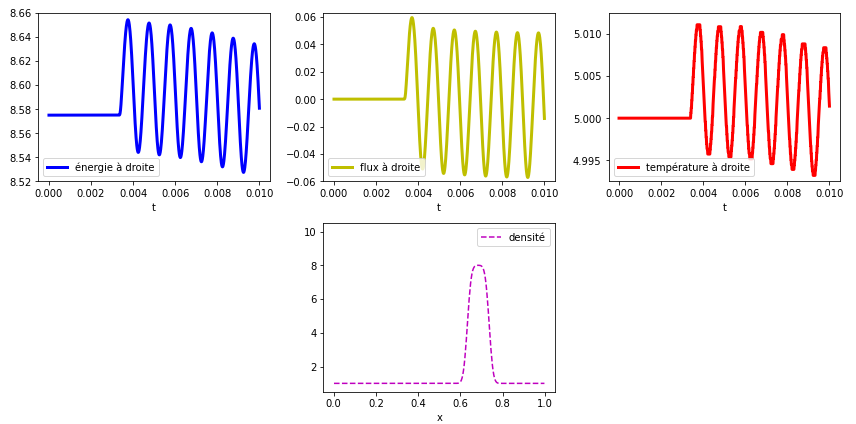
\includegraphics[width=.6\linewidth]{EntreeSortie1D} 
\decoRule
\caption[EntreeSortie1D]{Visualisation d'une entree (en haut) et d'une sortie (en bas) en 1D. Seul le signal sur la droite est utilise. Les 3 canaux E, F et T sont representes ici.}
\label{fig:EntreeSortie1D}
\end{figure}

En 1D, les entrees ne sont constituees que du signal recuperer sur le bord droit du domaine. La forme d'une example en presentee a la figure \ref{fig:Entrees1D}.

\begin{figure}[!h]
\centering
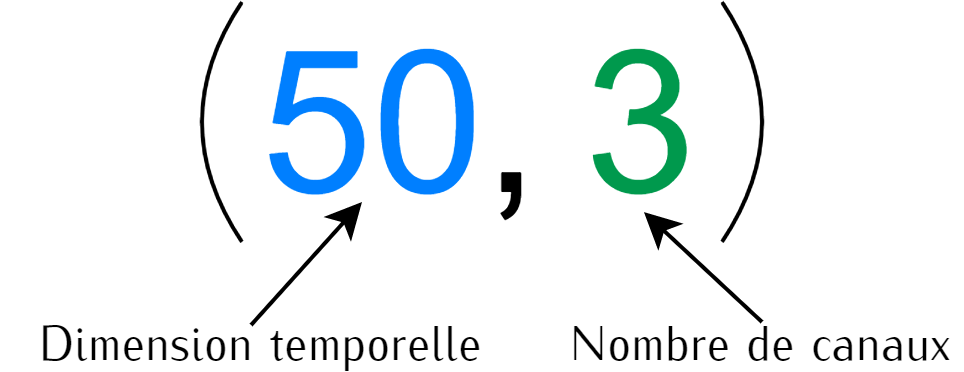
\includegraphics[width=.4\linewidth]{Entrees1D} 
\decoRule
\caption[Entrees1D]{Forme d'une entree en 1D. La dimension spatialle a ete reechantillonne de 907 a 50 iterations. Les 3 canaux designent les signaux E, F et T.}
\label{fig:Entrees1D}
\end{figure}

\subsection{En 2D}
Une entree 2D contient considerableme plus d'informatiosn. Les 3 signaux E, F et T sur les 4 bords y sont inclus. On y inclu aussi un signal correpondant a l'une des quatre positions de la source dans chacun de ces cas. En effet, une entree correspond a 4 simulations effectuees chacune avec la source a une position differente comme on peut le voire a la figure . Comparer a la 1D, il faut rajouter l'ordonnee du saut de densite pour obtenir la densite.

\begin{figure}[!h]
\centering
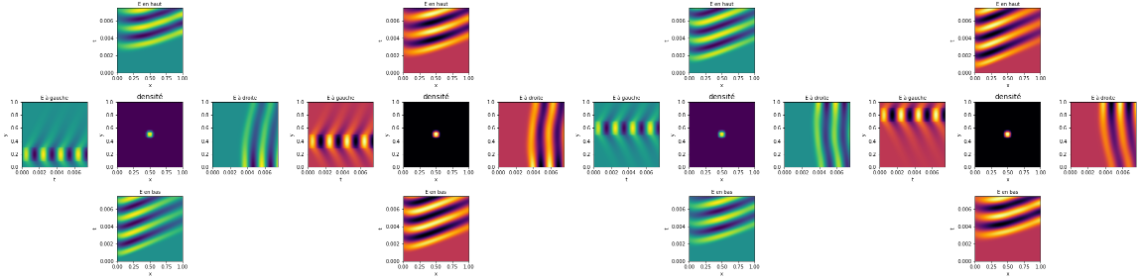
\includegraphics[width=.95\linewidth]{EntreeSortie2D} 
\decoRule
\caption[EntreeSortie2D]{Visualisation d'une entree (aux alentours des quatre images) et d'une sortie (aux mileiux) en 2D. On peut voire les postions des 4 sources utilisees a tour de role pour former une seule entree. Ici n'est representee que l'energie (qui constitue 1/3 des canaux) sur les 4 bords. Les images des densites presentee ci-contre ont ete obtenue par interpolation bilineaires d'une image initiale (28x28) moins fine.}
\label{fig:EntreeSortie2D}
\end{figure}


La forme d'une entree est representee a la figure \ref{fig:Entrees2D}. Des jeux de donnes complets 1D/2D ont ete sauvegardee et les details pour els recuperer et les traiter sont donnes en Anexe \ref{AppendixB}.

\begin{figure}[!h]
\centering
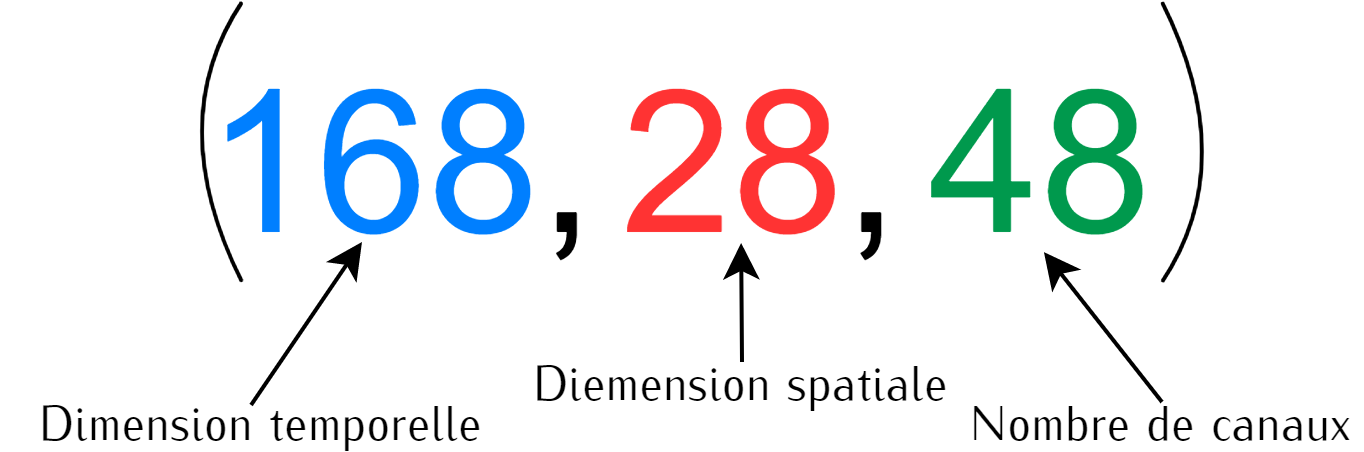
\includegraphics[width=.5\linewidth]{Entrees2D} 
\decoRule
\caption[Entrees2D]{Forme d'une entree en 2D. Contrairement a la 1D, il faut tenir compte de la dimention spatiale qui correspond au nombre de mailles sur chaque bords du domaine (N=M=28). Le nombre de canaux augmente donc considerablement. On passe a 48 car il faut tenir compte des 3 canaux originaux (E, F, et T), ensuite de chacun de 4 bords du domaine, et enfin des 4 positions de la source.}
\label{fig:Entrees2D}
\end{figure}

%----------------------------------------------------------------------------------------

\section{Architecture generale}

Un reseau de neuronnes artificel \footnote{nous y fereons reference dans la suite juste par reseau de neurones} est un systeme computationnel base sur le reseau de neuronnes biologique. L'apprentissage profond\footnote{definition du nombre de couche} permet de resoudre des problemes en Machine Learning\footnote{definition} que les methodes telles que la regression ineaire, etc.. ne peuvent pas. Il reussit cela en introduisant des representations des donnes qui s'exprimes sous forme d'autres representations, plus simples cette fois. Les reseaux profonds en aval\footnote{en oposition a un reseau de neurones recurrent qui reutilisent els resultats des model pour s'ameliorer} (ou MLP) consitituent l'exemples typique en apprentissage profond. Il s'agit juste d'une fonction (composition de differentes fonctions) faisant correspondre une serie d'entree a une serie de sortie $f^{-1} = composition de f1, f2, etc.$.

Un MLP est constitue de plusieurs couche (assimilables aux fonction f1, f2, .. precedentes) apprenant chacune un aspect particulier des donnnees (voir figure \ref{fig:MLP}. On distingue une couche d'entree, une ou pleusieurs couches cachees, et une coche de sortie).


\begin{figure}[!h]
\centering
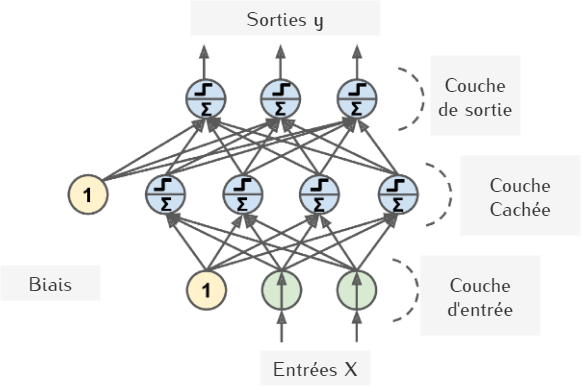
\includegraphics[width=.6\linewidth]{MLP} 
\decoRule
\caption[MLP]{Illustration d'un MLP avec une couche dense comme couche cachee. Le noombre de couche cachee peut etre elevee ce qui conduit aux reseaux de neurones profonds. Le 1 represente le biais \parencite[286]{Reference8}.}
\label{fig:MLP}
\end{figure}

Les reseaux de neurones convolutifs sont une forme de MLP spcialises dans le traitement des donnes qui ont une form de grille. Par exemple des series en temps qui peuvent etres vues comme des grilles 1D (l'axe de temps) prenant des donnes (vecteur de donnees) a interval de temps regulier \parencite{Reference5}. Ils sont donc particulieremt adaptes a la reconstruction de la densite partant des signaux temporels E, F, et T. L'archiytecture de base a ete proposee par M. Vigon. Nous utilisetons deux variantes: DRNN \footnote{Density Reconstruction Neural Network} 1 (figure \ref{fig:DRNN1}) et DRNN 2 (figure \ref{fig:DRNN2}).  Les architectures seront implemntee sous la librarie de machine leanring Keras (avec Tensorflow backend) Les differentes couches presentes seront detailles dans la suite. Nous indiquerons aussi en quoi elles sont importantes pour notre apprentissage.

% \begin{figure}[!h]
% \centering
% 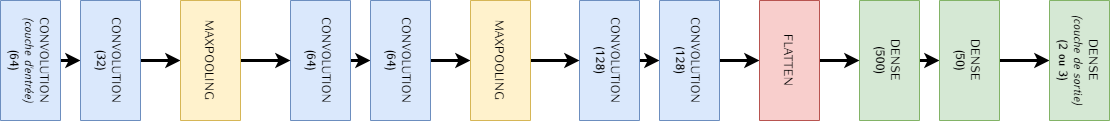
\includegraphics[width=.95\linewidth]{DRNN1} 
% \decoRule
% \caption[DRNN1]{Premeire architecture (nommee DRNN 1). Le nombre de neurnoes de la couche de sortie depend qu'on soit en 1D ou en 2D. Ce modlee contient pas des couche de Pooling\footnote{les details concernant le pooling seront donnes plus tard}. Le nombre de neurones utilises pour chaque couches est indiques entre parentheses}
% \label{fig:DRNN1}
% \end{figure}
% 
% \begin{figure}[!h] 
% \centering
% 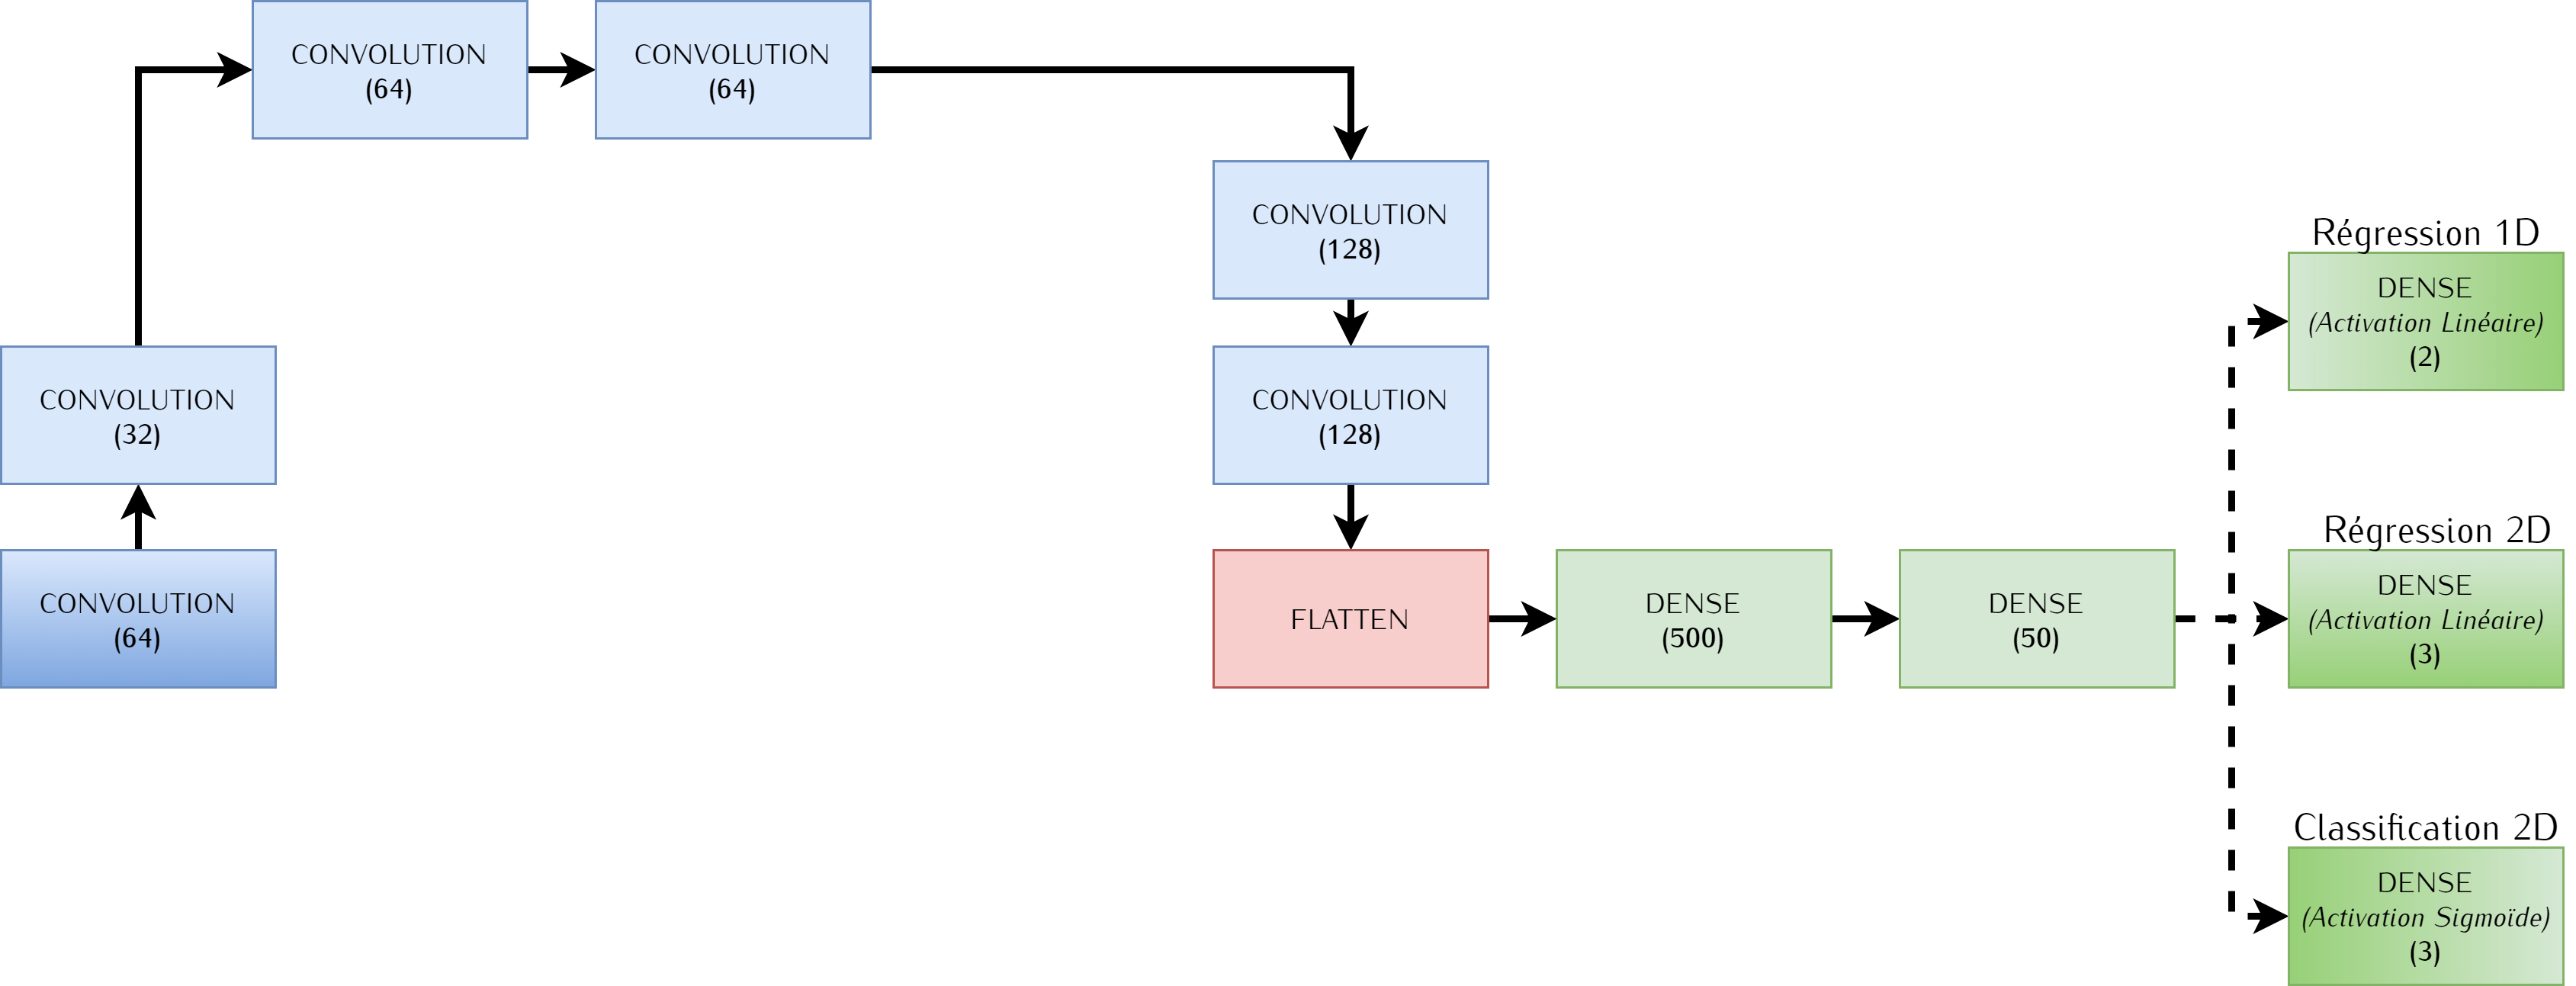
\includegraphics[width=.95\linewidth]{DRNN2} 
% \decoRule
% \caption[DRNN2]{Deuxieme architecture utilisee (nommee DRNN 2). Ce modlee ne contient pas de couches de Pooling}
% \label{fig:DRNN2}
% \end{figure}

\newpage
\begin{figure}[!ht]
   \begin{minipage}{0.6\textwidth}
     \centering
     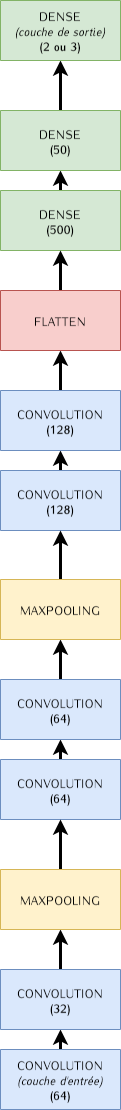
\includegraphics[width=.2\linewidth]{DRNN1ROT}
     \decoRule
     \caption[DRNN1]{Premeire architecture (nommee DRNN 1 ). Le nombre de neurones utilises pour     
     chaque couches est indiques entre parentheses. Le nombre de neurnoes de la couche de sortie 
     depend qu'on soit en 1D ou en 2D.}
     \label{fig:DRNN1}
   \end{minipage}\hfill
   \begin{minipage}{0.4\textwidth}
     \centering
     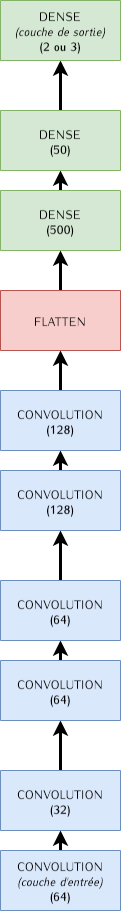
\includegraphics[width=.3\linewidth]{DRNN2ROT}
     \decoRule
     \caption[DRNN2]{Deuxieme architecture utilisee (nommee DRNN 2). Ce modlee ne contient pas de 
     couches de Pooling \footnotemark }
     \label{fig:DRNN2}
   \end{minipage}
\end{figure}
\footnotetext[6]{Les details concernant l'operation de "pooling" seront donnes a la section \ref{subsec:MaxPoling}}

% \begin{figure}[!ht]
% \begin{subfigure}{.6\textwidth}
%   \centering
%   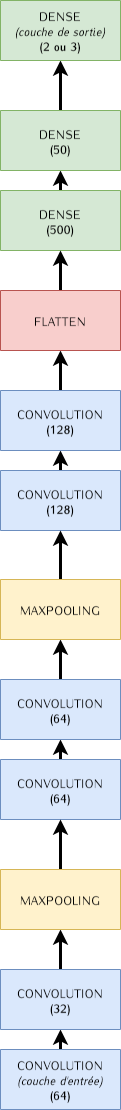
\includegraphics[width=.2\linewidth]{DRNN1ROT}  
%   \caption[DRNN1]{CPremeire architecture (nommee DRNN 1 ). Le nombre de neurones utilises pour     
%      chaque couches est indiques entre parentheses. Le nombre de neurnoes de la couche de sortie 
%      depend qu'on soit en 1D ou en 2D.}
%   \label{Fig:DRNN1}
% \end{subfigure}
% \begin{subfigure}{.4\textwidth}
%   \centering
%   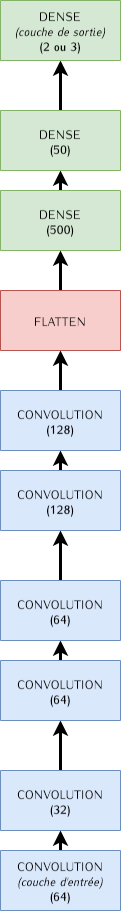
\includegraphics[width=.3\linewidth]{DRNN2ROT}  
%   \caption[Conv2D]{Deuxieme architecture utilisee (nommee DRNN 2). Ce modlee ne contient pas de 
%      couches de Pooling \footnote{Les details concernant le pooling seront donnes a la section \ref{subsec:MaxPoling}}}
%   \label{Fig:DRNN2}
% \end{subfigure}
% \label{Fig:DRNN}
% 
% \centering
% \decoRule
% \caption[DRNN]{Differents modeles de CNN utilises}
% \end{figure}
% 

----------------------------------------------------------------------------------------

\section{Les couches utilisées}

\subsection{Les couches de convolution}
la convolution est l'operation fondamentale d'un CNN. Il s'agit d'une operation lineaire qui combine deux signaux pour en extraire un troisieme. En general, une operation de convolution se definit par la formule suivante (i est le ssignal d'entree et k est le noyau de la convolution)
$$ s(t) = (i * k)(t) = \int i(x)k(t-x) \, dx $$

En pratique, les signaux temporels ne sont pas continus, ils sont discretises par interval de temps $\Delta t$. Dans ce contexte, la convolution 1D se definit par la formule:
\begin{equation}
 s(t) = \sum_{x=-\infty}^{\infty} i(x)k(t-x)
 \label{eqn:Conv1D}
\end{equation}

Cette formule doit aussi etre adaptee en 2D vu que nos inputs sont 2D. La formule devient donc:
\begin{equation}
 S(i,j) = (I * K)(i,j) = \sum_{m}\sum_{n} I(m,n)K(i-m,j-n)
 \label{eqn:Conv2D}
\end{equation}

L'operation de convolution est commutative grace a l'inversion du noyaux relativement au siganal d'entree. Cette propriete, bien qu'importante d'un point de vu therique, ne prensente pas d'avantages majeure du point de vu computationnel. C'est la raison pour laquelle on dispose de l'operation de cross-correlation qui est convolution sans inversion du noyau. En 2D elle se presente comme ceci:
\begin{equation}
 S(i,j) = (I * K)(i,j) = \sum_{m}\sum_{n} I(i+m,j+n)K(m,n)
 \label{eqn:Corr2D}
\end{equation}

On remarque aussi que le parcours des indices se fait suivant l'input. Il se trouve que c'est plus direct et rapide ainsi, parcequ'il y a moins de varaition dans la plage de valeurs valides pour $n$ et $m$. 

Plueieurs libraries de machine leanring implementent la cross-corelation mais l'appellent convolution. C'est le cas de Keras lorsqu'elle utilise le backend Tensorflow \footnote{Lorsqu'on utilise Theano, les convolutions sont effectivement des convolution comme definie en \ref{eqn:Conv1D} et \ref{eqn:Conv2D}} \parencite{Reference6}.
% 
% \begin{figure}[!h]
%     \subfloat[Convolution 1D]{
%    \begin{minipage}{0.5\textwidth}
%      \centering
%      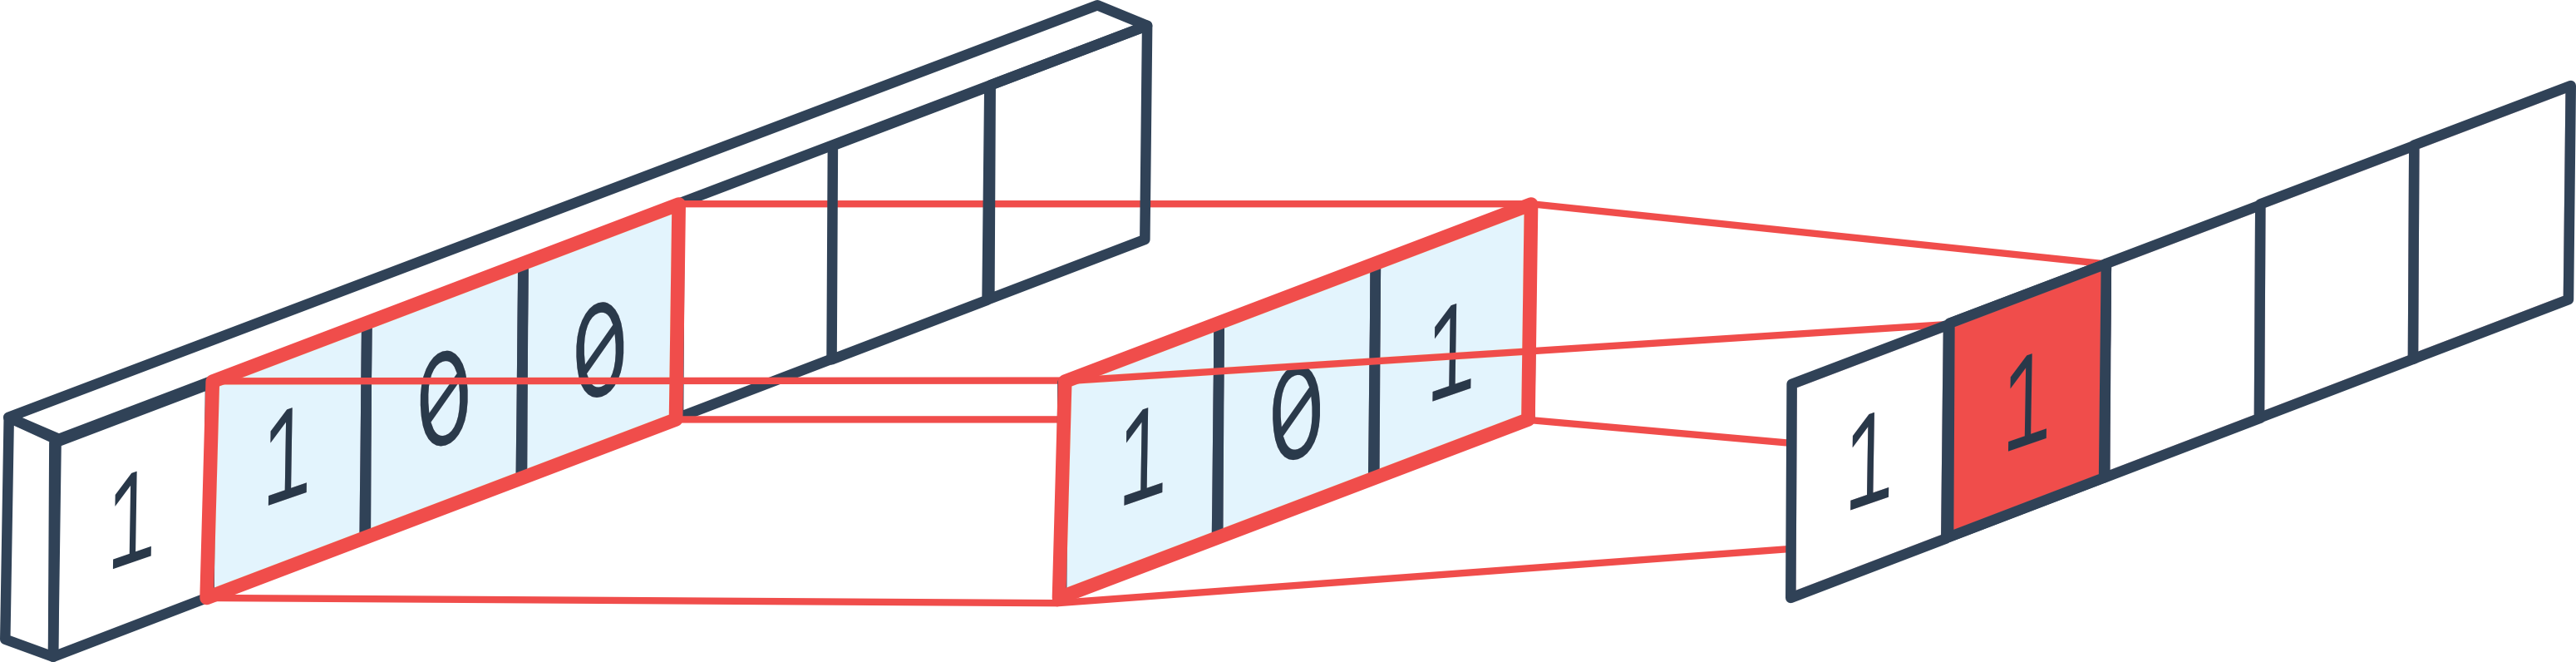
\includegraphics[width=.95\linewidth]{Conv1D}
%    \end{minipage}}
%    \hfill
%    \subfloat[Convolution 2D]{
%    \begin{minipage}{0.5\textwidth}
%      \centering
%      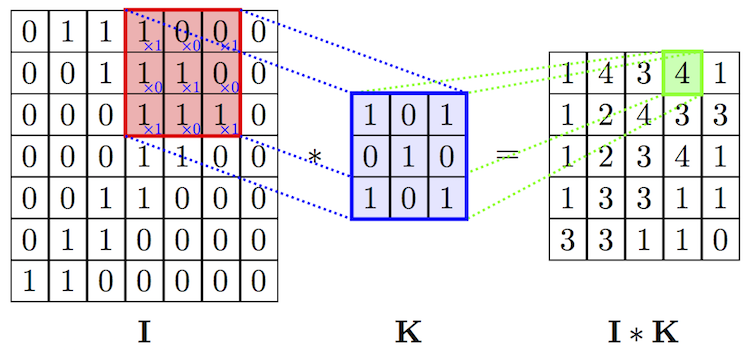
\includegraphics[width=.95\linewidth]{Conv2D}
%    \end{minipage}}
%    \label{Fig:Conv1D2D}
% 
%    \centering
%    \decoRule
%    \caption[Conv2D]{Illustration d'une convolution (cros-corelation) 1D/2D en mode "valide" (aucun padding de 0 ne sera ajoute et la sortie S aura une taille inferieure a l'entree I). La taille du noyaux que nous utiliserons sera de 3 (1D) et (6,2) (2D) . Un autre paramtre important pour reduire la taille de la sortie est le "stride", il s'agit de l'ecart entre deux applications du noyaux de convolution K. Nous le prenons egale a 1 (1D) et (1,1) (2D) de facon a couvrir tous les indices valides de l'entree I.}
% \end{figure}


\begin{figure}[!h]
\begin{subfigure}{.5\textwidth}
  \centering
  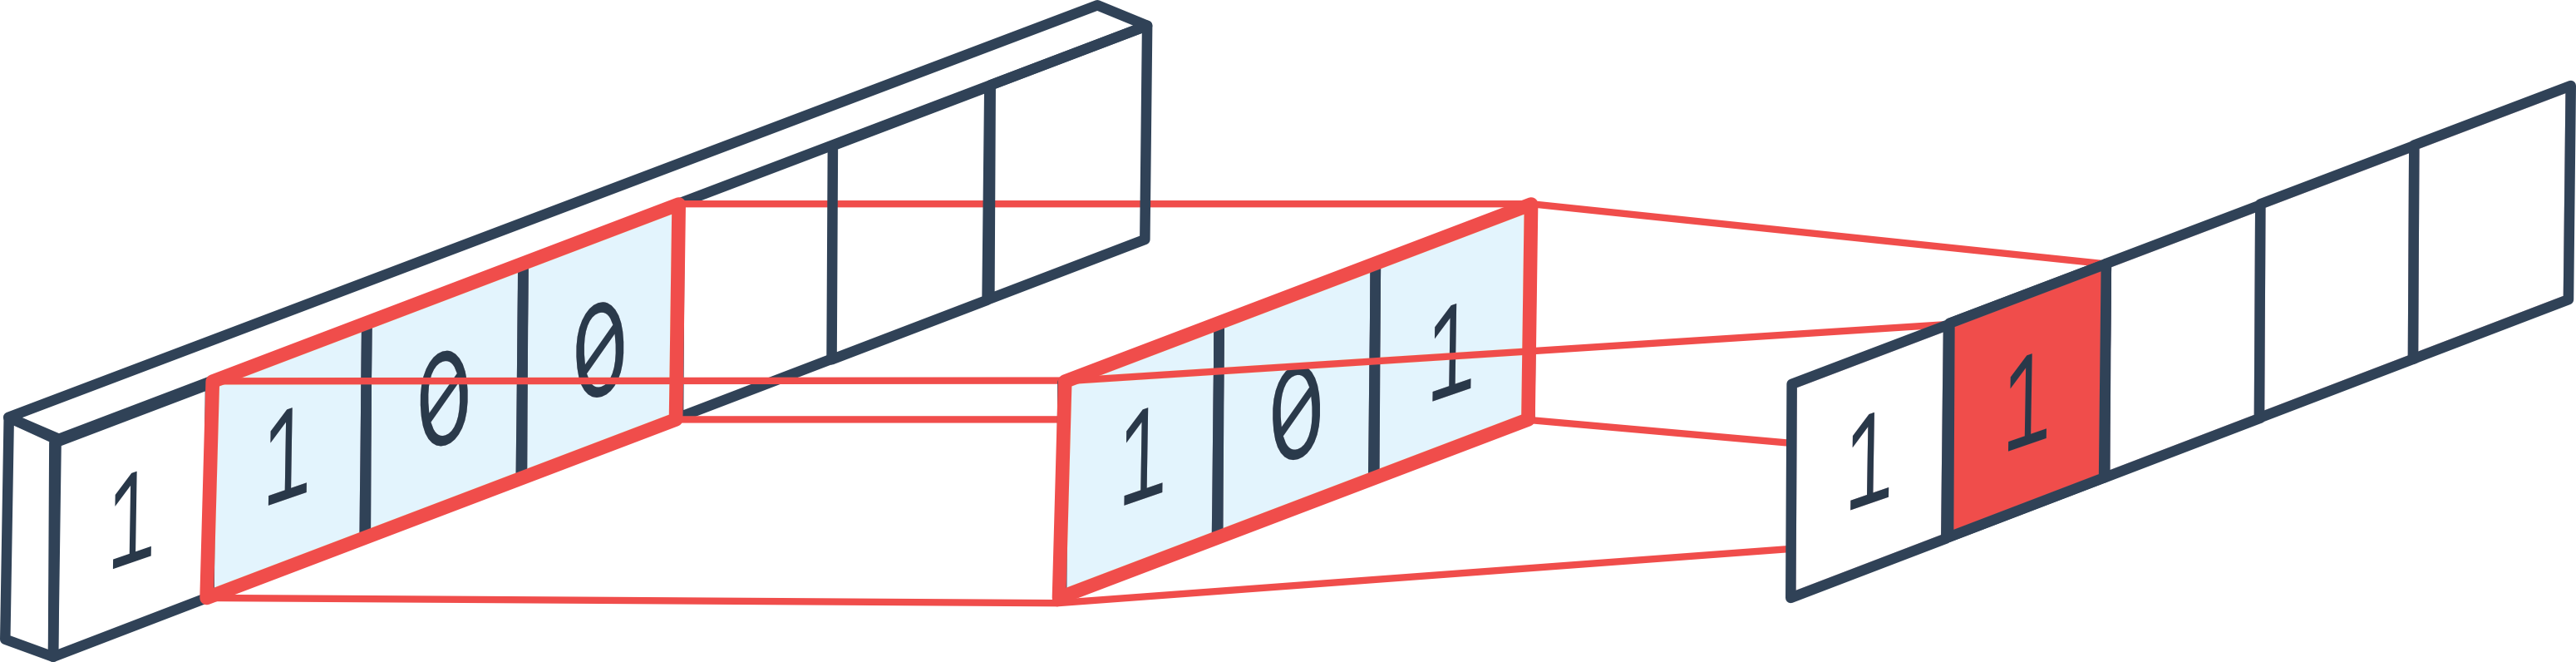
\includegraphics[width=.95\linewidth]{Conv1D}  
  \caption[Conv1D]{Convolution 1D \parencite{Reference10}}
\end{subfigure}
\begin{subfigure}{.5\textwidth}
  \centering
  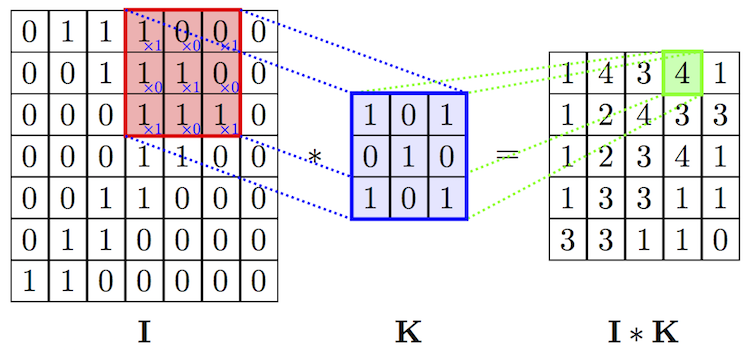
\includegraphics[width=.95\linewidth]{Conv2D}  
  \caption[Conv2D]{Convolution 2D \parencite{Reference11}}
\end{subfigure}
\label{fig:Conv1D2D}

\centering
\decoRule
\caption[Convolution1D2D]{Illustration d'une convolution (cros-corelation) 1D/2D en mode "valide" (aucun padding de 0 ne sera ajoute et la sortie S aura une taille inferieure a l'entree I). La taille du noyaux que nous utiliserons sera de 3 (1D) et (6,2) (2D) . Un autre paramtre important pour reduire la taille de la sortie est le "stride", il s'agit de l'ecart entre deux applications du noyaux de convolution K. Nous le prenons egale a 1 (1D) et (1,1) (2D) de facon a couvrir tous les indices valides de l'entree I.}
\end{figure}



% 
% Les CNN apportent trois notions cles a un apprentissage:
% \begin{itemize}
%  \item l'interaction creuse: contrairemetn aux couches traditionneles, les couches de convolution utilisent des noyaux de taille condiereblemen inferieure a celle de l'input. En terme de multiplication matricielle, cela permet de faire des taches toutes aussi importantes (detection des condouts, floutage, etc..) en ne gardant que peu de parametres en memoire et augmentant l'efficacite statitique. Cela permet aussi de reduire les couts de calcul.
%  (IMAGE)
%  \item le partage des parametres: les coefficient du noyau de convolution sont reutilises a chaque endroit de la matrice d'entree, contrairement aux couches traditionnelles qui utilise generalement chaque coefficient une seule fois.
%  (IMAGE)
%  \item la representation equivariante: le partage de parametre introduit la proprite d'equivaraition par translation. SI l'entree change, la sortie change de la meme facon, et le reseau de neurones exploite cela. Par exemple, dans l'etude d'une image, il serait interressant de detecter les contour dans la premiere couche du reseau,vu que ces meme contour sont suceptibles de reaparatire dans la suite. (\parencite{Reference5})
% \end{itemize}


Dans les architecture de CNN typiques, la couche de convolution est generalement suivi d'une etape dite de detection. Dans cette etape, les resultas lineaires de la convolution sont passes a une fonction non lineaire auniveau d'une couche de d'activaiotn. Nous detaillerons les details de l'activation dans les sections suivantes. Apres cette etape de detection, le Pooling est generalement applique pour modifier les resulats encore plus profoncdement.

\subsection{Le MaxPoling}
\label{subsec:MaxPoling}
L'operation de Pooling permet de reduire la taille des donnees (downsampling). Une fonction de pooling tranforme les entres voisines par une fonction d'aggregation statistique. Plusieurs fonctions d'aggregations peuvent etres utlisees. Par examples, le maxpooling renvoi le maximum parmis les entrees sur un domaine (rectigne en 1D et rectangulaire en 2D). 


\begin{figure}[!h]
\begin{subfigure}{.5\textwidth}
  \centering
  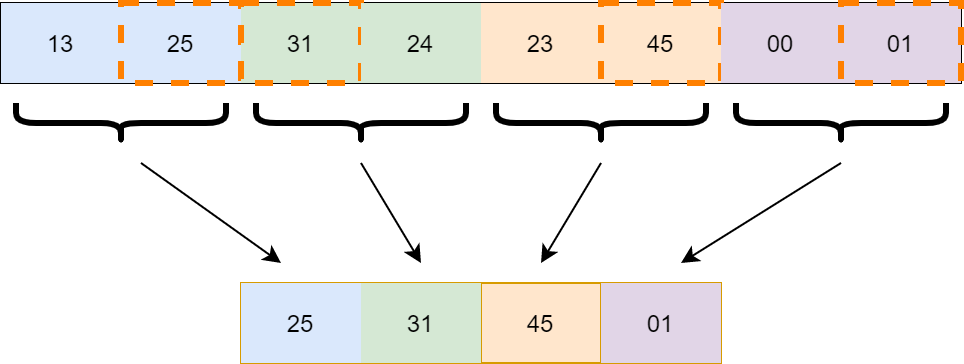
\includegraphics[width=.95\linewidth]{MaxPool1D}  
  \caption[MaxPool1D]{Maxpooling 1D}
\end{subfigure}
\begin{subfigure}{.5\textwidth}
  \centering
  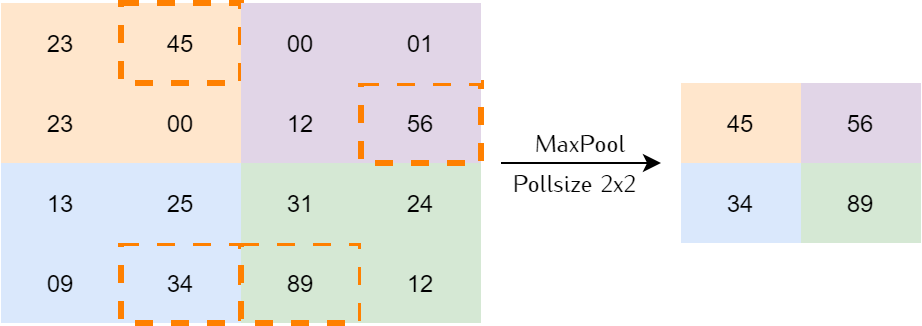
\includegraphics[width=.95\linewidth]{MaxPool2D}  
  \caption[MaxPool2D]{Maxpooling 2D}
\end{subfigure}
\label{fig:MaxPool1D2D}

\centering
\decoRule
\caption[MaxPoling]{Operatioon de maxpooling en 1D/2D avec un "pool size" de 2 (en 1D) et de 2x2 (en 2D)}
\end{figure}


En general, l'operation de pooling permet de rendre la representation approximativemtn invariante aux petite variatons dans l'input. Parlant de l'identifcation d'objects dans une image par exemple, \textit{l'invarianve par translations locales (petites tranalations) peut etre utile si on est plus interresse par la presence de l'object que par sa localisation exacte}\parencite[321ff.]{Reference5}.

Dans le probleme inverse que nous resolvons, on est aimerais non seulement detecter la presence du saut de densite, mais aussi ses coordonnes exactes. Cela nous amenera donc a considerer dans un premier temps une architecture avec pooling (figure \ref{fig:DRNN1}), et dans un dexieme temps, sans Pooling (figure \ref{fig:DRNN2}).
 
\subsection{Flatten}
L'operation d;applattissage permet de transformer les donnees en quittant de la forme tensorielle (2D avec plusieurs canaux) a une forme vectorielle. Il s'agit en realite d'une etape de preparation a une couche complement connectee.

\begin{figure}[!h] 
\centering
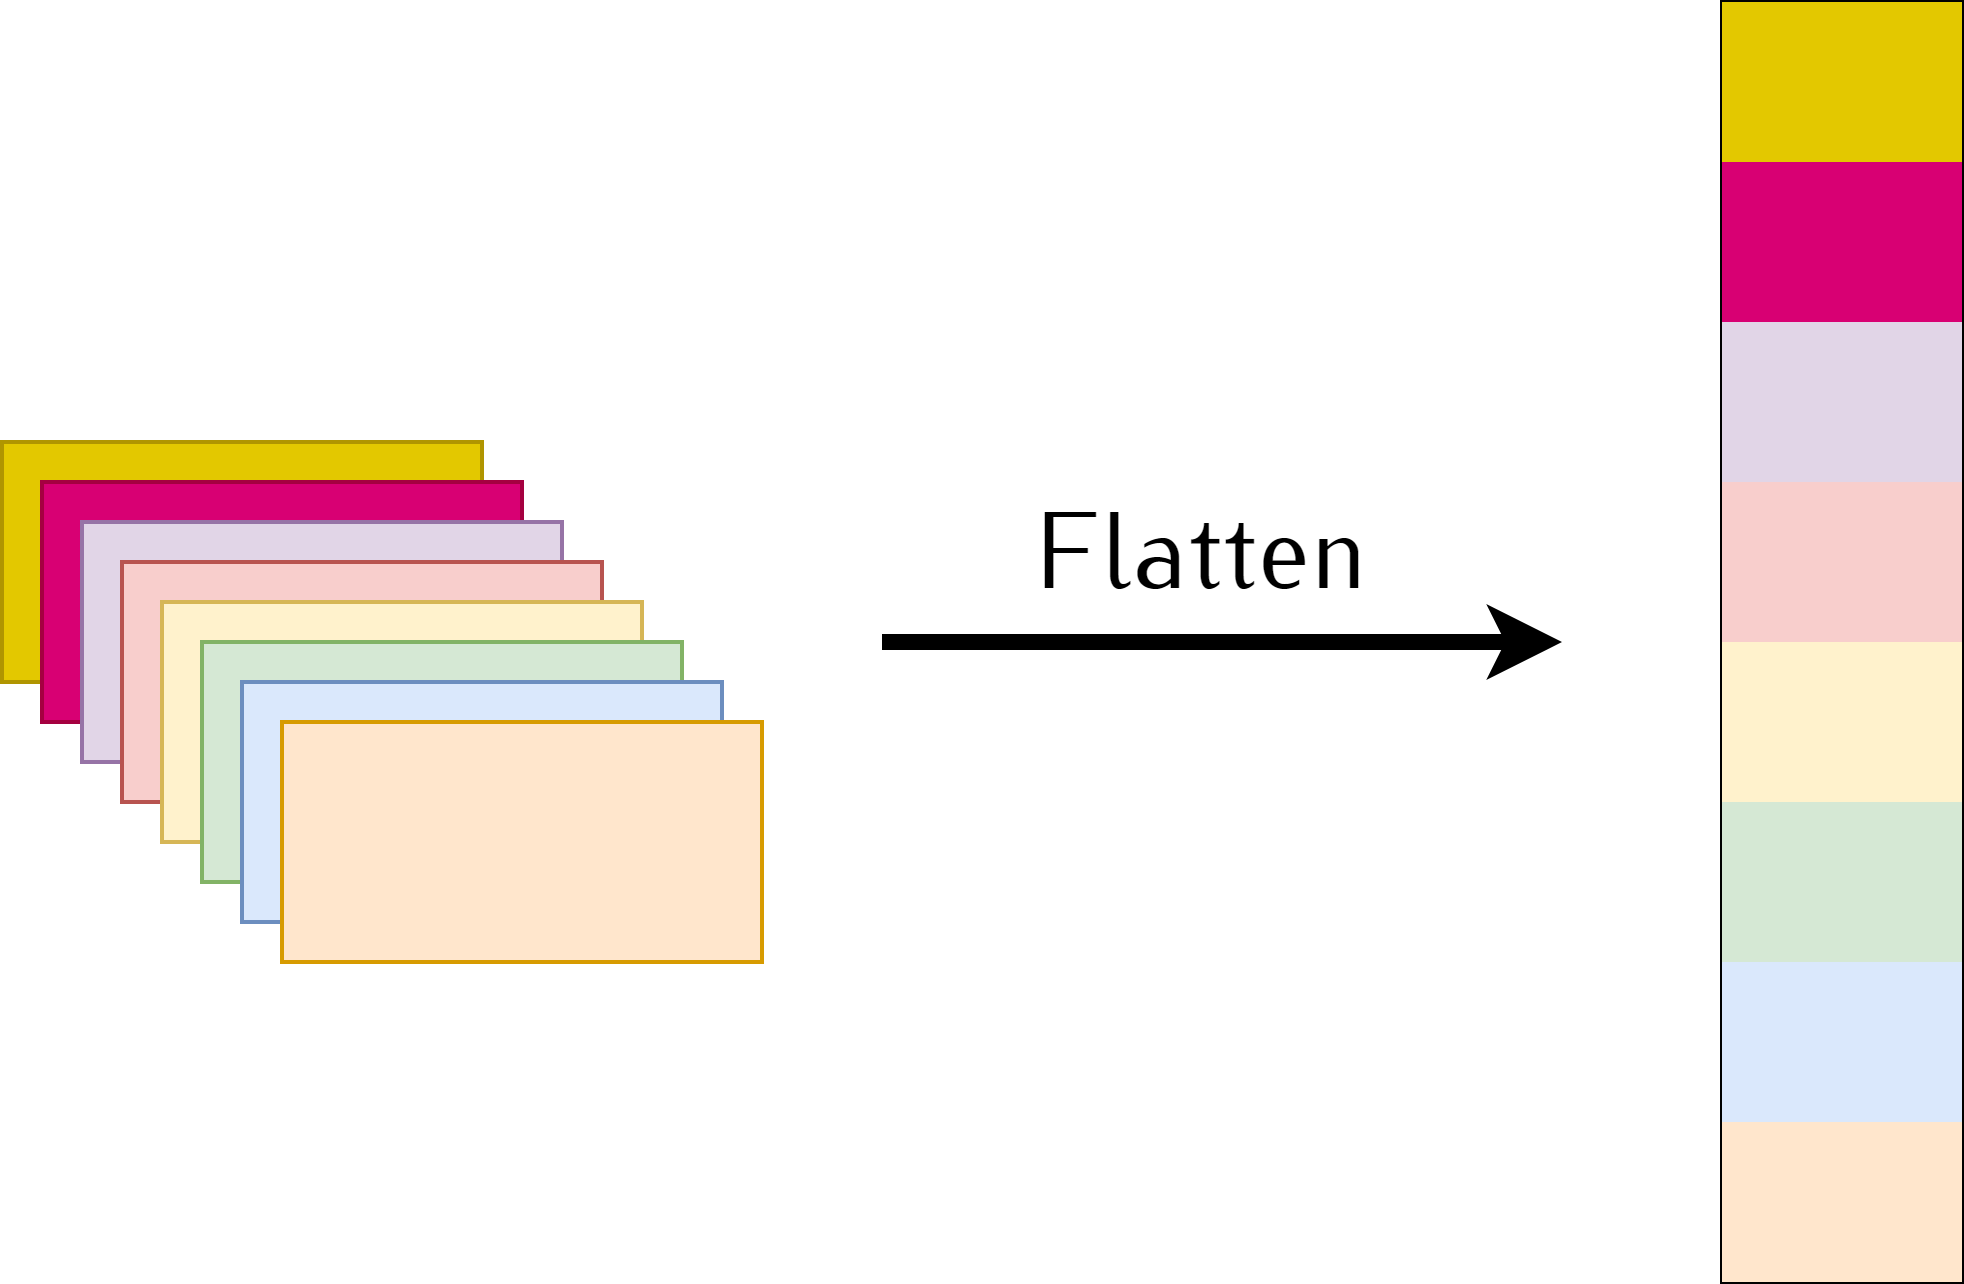
\includegraphics[width=.5\linewidth]{Flatten}
\decoRule
\caption[Flatten]{Illustration d'une operation de flatten). Qu'on soit en 1D ou en 2D, le flatten assure que la sortie est un vecteur sur lequel une couhe Dense peut operer.}
\label{fig:Flatten}
\end{figure} 

\subsection{Les couches denses}
Dans cette couche, tous les neurones sont connectes a tous les neurones de la couche precedente. Une couche dense prend les resultats d'une convolution/pooling et en resort des poinds. Les couches de convolution ayant apris des aspects particuliers des donnees, la couche est un moyen facile d'apprndre des combinaisons non lineaires de ces dernieres.

Si $f_2$ designe la fonction representant une couche dense. l'operation efffectuee est la suivante: $f_2=\phi(XW+b)$, ou $X$ represente les entrees de la couche, $b$ le bias , $W$ la matrice des poinds (une ligne par neurone d'entree et une colone par neurone de cette couche, excepte ceux du biais), et $\phi$ designe la fonction d'activation que nous detaillerons plus tard. \parencite[286]{Reference8}

\begin{figure}[!h] 
\centering
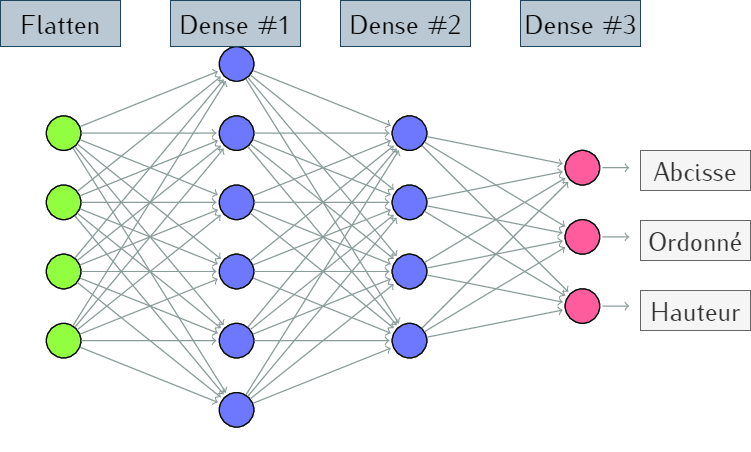
\includegraphics[width=.5\linewidth]{Dense} 
\decoRule
\caption[Dense]{Serie de 3 couches denses "fully connected". La couche (en vert) represent le resultat de l'opeation de Flatten. L'utilisation des couches denses constitue la derniere etape des reseax en figures \ref{fig:DRNN1} et \ref{fig:DRNN2}(Image adaptee de \parencite{Reference9})}
\label{fig:Dense}
\end{figure}

%----------------------------------------------------------------------------------------

\section{Configurations de l'entrainement sous Keras}
Keras proposent une multitude d'otions et d'hyperparatres pour tuner le modele. Les plus importants sont detailles dans les sections suivantes.

\subsection{Les hyper-parametres}

\subsubsection{L'optimiseur}
L'optimization est une methode d'acceleration de l'entrainement. L'optimiseur Adam\footnote{Adaptative moment estimation} combine les proprietes de deux autres algorithmes d'entrainement (AdaGrad et RMSProp).

\subsubsection{Activation RELU}
La fonction d'activation introduit une non-linearite entre les couche. L'avatage majeure de l'activation ReLU\footnote{Rectified Linear Unit} par rapport aux autres fonctions d;activation c'est qu'il n'active pas tous les neurones en meme temps. D'un pooint de vue computationel, elle est tres eficace tout en produidant des resulats satisfaisants.

\subsubsection{le taux d'apprentissage}
Il s'agit du parametre le plus influant pour notre apprentissage. Il controle a quelle vitesse le modele \footnote{les poids des neurones sont initialises de facon aleatoire} s'adapte au probleme en determinant de quelle quantite les poids des neurones seront mis a jour apres l'agorithme de backpropagation. S'il est tres eleve, il raoidement conduire a solution non optimale; s'il est tres faible, le modele peut reste fige (il fadra alors un nombre eleve d'epoques pour le debloquer).

Avec un taux d'apprentissage egale a 1e-4, nous n'avons ete capable que de detecter la hauteur du crenau en 1D; et une reduction supplementaire entraine la divergence du modele. En 2D, il a fallu descendre jusqua 1e-5 pour determiner avec precision l'abcisse, l'ordonne, et la hauteur du crenau.

\subsubsection{le batch size}
Il s'agit de la taille de chauque paquet de donnnes \footnote{nombre d'instaces d;entrainement selectiones aleatoiremetn} passes au modele durant un epoque. Un batch size faible apporte du bruit au modele vu qu'une partie aleatoire des donnes est tulisee pour mettre ajour les poids des neurones. Ceci permet une meilleure generalisation du modele tout en permettant une limiter la quantite de donnees chargee dans la RAM a chaque epoque.

% 
% \subsubsection{le coefficient de reglarisation L2}
% Le penalisation permet d;eviter le surapprentissage. Sous Keras, on peut soit penaliser les poids d'une couche (kernel optimizer), ou bien penaliser les resultats de la fonction d'activation de cette couche (activity optimizer). la deuxieme option a offert les meilleures resultats, c'est pourquoi l'avons appliquee a nos deux couches de neuronnes denses  de nos modeles avec un coefficient de 1e-5.
% 

\subsubsection{Early stopping}
La technique d'early sera notre moyen primaire de lutte contre le sur-appretisage. Pour l'implementer de facon efficace sous Keras, il nous faut une \verb|patience|. Il s'agit du nombre d'epoques a attendre avant d'areter d'areter l'apprentissage de facon precosse. Nous arreterons nos entrainement des que le score R2 (voir paragraphe \ref{subsub:R2}) sur le jeu de validation n'aura pas augmente pendant 10 epoques. 

\subsection{Les metriques}

\subsubsection{Loss MSE}
Pendant la generation des donnees, on a pris soin de pas introduire de donnes aberantes. La MSE qui est plus elevee sur les valeurs aberantes que la MAE est dont plus adaptee ici. Si les $\hat{y}_i$ designent les predictions et $y_i$ les veritables cibles (valeurs observees), la MSE se definit par:
\begin{equation}
 MSE = \frac{1}{n} \sum_{i=1}^{n} \left( y_i - \hat{y}_i \right)^2
 \label{eqn:MSE}
\end{equation}

\subsubsection{Coefficient de determination R2}
\label{subsub:R2}
Le Coefficient de determination R2 est tres important en statistique. On peut l'obtenir par la formule:
\begin{align}
 R^2 = 1 - \frac{SS_{res}}{SS_{tot}}
 \label{eqn:R2}
\end{align}
Avec
\begin{align*}
 \quad SS_{res} =  \sum_{i=1}^{n} \left( y_i - \hat{y}_i \right)^2 \quad \text{et} \quad SS_{tot} =  \sum_{i=1}^{n} \left( y_i - \bar{y} \right)^2 
\end{align*}
Ou $ \bar{y} = \sum_{i=1}^{n} y_i $ represente la moyenne des valeurs observees.

On peut remarquer que:
\begin{itemize}
 \item Si le modele predit les valeurs attendues (observees), le score R2 vaut 1. 
 \item SI le modele predit toujours la valeur moyenne $\bar{y}$, le score R2 vaut 0
 \item Si les predictions sont pires que la moyenne, le score R2 est negatif
\end{itemize}

En generalOn voit que si les predictions et les valeurs observees sont tres correles (sans etre egaux), on aura un score R2 ce qui n'est pas carateritique des resultats. En effet, pour des taches de regression il se definit comme etant le caree du coefficient de correlation entre les valeurs predites et les valeurs observees.

Dans la suite de ce rapport, le score R2 sera presente sous forme de pourcentage. 

\subsubsection{Un score personalise}
On definit donc un nouveau score particulieremtn adapte a nos donnees. On decalre qu'une prediction est correcte si elle est suffisament proche du label:
\begin{itemize}
 \item au dizième près pour la position (suivant x ou y) car le domaine de d'etude est $[0,1] \times [0,1]$
 \item à l'unité près pour la hauteur car les hauteurs observees sont comprises entre 0 et 10
\end{itemize}

Le score personalise est un score severe (pourcentage de prediction correctes) qui qui recompense les prediction qui sont a la fois precisent en hauteurs et en position. La prediction de la position etant le probleme majeure auquel nous avons fait face, il cause generalement des valeurs faibles pour le score personalise.

%----------------------------------------------------------------------------------------

\section{Resultats}

Nous resumons la sections precedentes en specifiant les paramtres (et leurs noms) utilises pour entrainer le modele sous Keras.

\begin{table}[h!]
\caption{Liste des parametres majeurs utilises pour l'entrainement. L'activation relu est utilisee sur les couches cachees et "linear" sur la couche de sortie}
\label{tab:Parametres}
\centering
\begin{tabular}{l l l}
\toprule
\tabhead{Parametre} & \tabhead{Definition} & \tabhead{Valeur 1D / 2D} \\
\midrule
\verb|learning_rate| & taux d'appentissage & 1e-4 / 1e-5\\
\verb|batch_size| & taille d'un batch a chaque epoque  & 32\\
\verb|optimizer| & algorithme d'optimisation & Adam\\
\verb|activation| & type de fonction d'activation  & "relu" ou "linear"\\
\verb|patience| & patience pour l'\verb|early_stopping| & 10\\
\verb|epochs| & nombre d'epoques & 100\\
\verb|kernel_size| & taille du noyau de convolution & 3 / (6,2)\\
\bottomrule\\
\end{tabular}
\end{table}


Nous avons entraine les architectures en 1D (fig ...) et par la suite en 2D (fig ...) en ajustant les dimensions des coushes de neurones connablement.

\subsection{Régression}
% 
    \subsubsection{En 1D}
    On obtient de tres bonnes predictions sur la hateur de l'obstacle qui affecte directement l'amplitude des signaux sur le bord droit du domaine. Ce score n'est pas assez indicatif vu que les predictions sur la position du crenaux ne sont pas assez precises. Le score personalise permet de capturer ce defaut et donne environ 25\%.
    
    Le modele avec MaxPoling correspond a la figure \ref{fig:DRNN1}, et celui sans MaxPooling a la figure \ref{fig:DRNN2}.
    
    
    \begin{table}[h!]
    \caption{Resultats obtenus sur le jeur de test en 1D. Ces valeurs representent une moyenne obtenue sur plusieurs cycles d'entrainement/prediction}
    \label{tab:Tab1D}
    \centering
    \begin{tabular}{l l l}
    \toprule
    \tabhead{Score} & \tabhead{Avec MaxPooling} & \tabhead{Sans MaxPooling} \\
    \midrule
    R2 & 99.49 \% & 99.50 \%\\
    personalise & 26.50 \% & 28.21 \%\\
    \bottomrule\\
    \end{tabular}
    \end{table}

    \begin{figure}[!h]
    \begin{subfigure}{.5\textwidth}
    \centering
    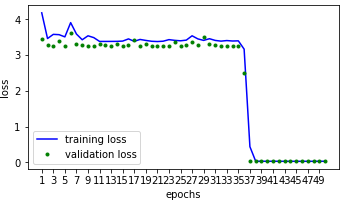
\includegraphics[width=.8\linewidth]{1DPool}  
    \caption[2DPool]{1D Avec Pooling}
    \end{subfigure}
    \begin{subfigure}{.5\textwidth}
    \centering
    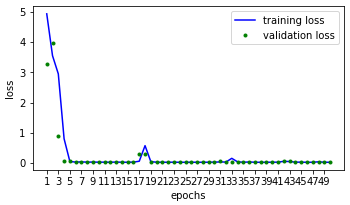
\includegraphics[width=.8\linewidth]{1DNoPool}  
    \caption[2DNoPool]{1D Sans Pooling}
    \end{subfigure}
    \label{fig:1DLoss}

    \centering
    \decoRule
    \caption[Loss 1D]{Comparaison de la vitesse de decroissiance de la loss en 1D}
    \end{figure}

    Meme si aucun n'est capable de correctement predire la position du crenau, le modele sans MaxPooling semble mieux se comporter sur ce jeu de donnees particulier. Pour les illustrations qui vont suivre, nous utilisetons donc ce dernier modele. Nous commencons par une illustration de la correlation entre les labels (valeurs observees) et les predictions (figure \ref{fig:Illustration1D}).
    
    \begin{figure}[!h]
    \begin{subfigure}{.5\textwidth}
    \centering
    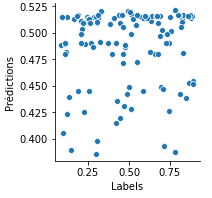
\includegraphics[width=.5\linewidth]{Position1D}  
    \caption[Pos1D]{Position}
    \end{subfigure}
    \begin{subfigure}{.5\textwidth}
    \centering
    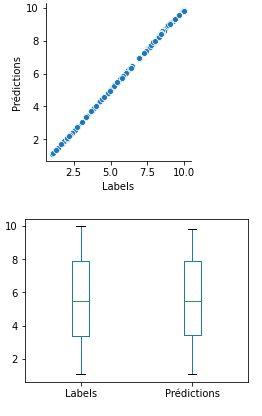
\includegraphics[width=.5\linewidth]{Hauteur1D}  
    \caption[H1D]{Hauteur}
    \end{subfigure}
    
     \centering
    \decoRule
    \caption[Illustration 1D]{Illustration de la correlation entre les labels et les predictions obtenues par le modele sans max-pooling en 1D. On peut observer l'exactitude des predictions pour la hauteur mais un echec sur la position. En effet, les predictions de la postion du crenau sont concentree autour de la moyenne 0.5}
    \label{fig:Illustration1D}
    \end{figure}

    Pour observer les meilleures et les pires predictions du modele, ils nous faut une mesure de la distance entre les predictions et les labels. On definit donc la norme ci-bas (en prenant soins de normaliser la hauteur). $$ \text{Norme} = \sqrt{\text{Position}^2 + \left( \frac{\text{Hauteur}}{10} \right)^2}$$
    
    Observons donc les meilleures predictions du modele (sans Maxpooling) (figure \ref{fig:Meilleur1D}).
    \begin{figure}[!h]
    \begin{subfigure}{.5\textwidth}
    \centering
    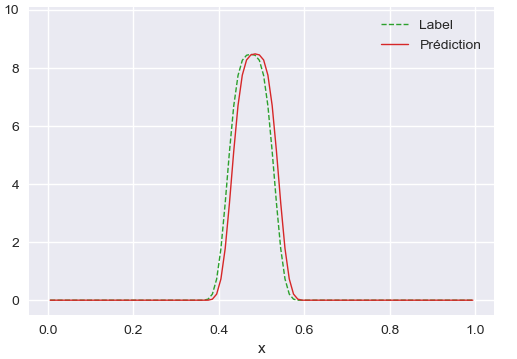
\includegraphics[width=.8\linewidth]{Meilleur1D1}  
    \caption[Meilleur1D1]{Label = [0.488 8.474] et Prediction = [0.49  8.486]}
    \end{subfigure}
    \begin{subfigure}{.5\textwidth}
    \centering
    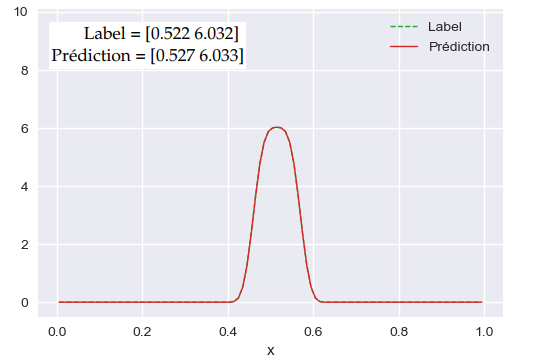
\includegraphics[width=.8\linewidth]{Meilleur1D2}  
    \caption[Meilleur1D2]{Label = [0.522 6.032]  et Prediction = [0.527 6.033]}
    \end{subfigure}
    
     \centering
    \decoRule
    \caption[Meilleur 1D]{Les meilleures predictions 1D. Il s'agit ici d'une reconstruction manuelle de la densite a partir des vecteurs presentes en (A) et (B). La premiere coordonne indique la position du saut de densite, et la deuxieme sa hauteur. On confirme que les bonnes predictions des positions sont proches du mileieu du domaine}
    \label{fig:Meilleur1D}
    \end{figure}
    
    Les pires predictions du domaine permettent de mieux illustrer les problemes rencontre avec l'apprentissage 1D (\ref{fig:Pire1D}).
    
    \begin{figure}[H]
    \begin{subfigure}{.5\textwidth}
    \centering
    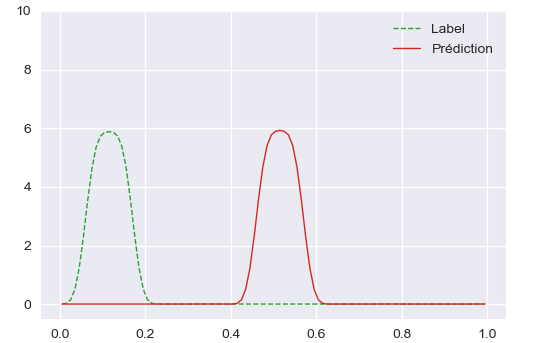
\includegraphics[width=.8\linewidth]{Pire1D1}  
    \caption[Pire1D1]{Label = [0.125 5.886] et Prediction = [0.524 5.925]}
    \end{subfigure}
    \begin{subfigure}{.5\textwidth}
    \centering
    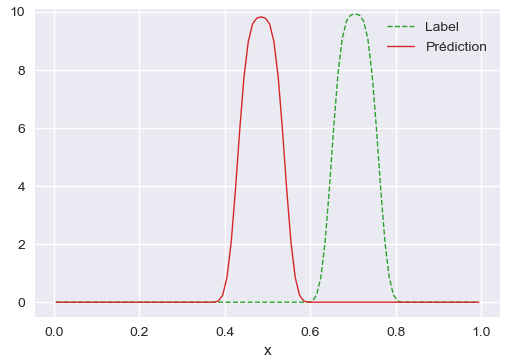
\includegraphics[width=.8\linewidth]{Pire1D2}  
    \caption[Pire1D2]{Label = [0.892 8.195]  et Prediction = [0.454 8.167]}
    \end{subfigure}

     \centering
    \decoRule
    \caption[Pire1D]{Les pires prediction du modele (sans MaxPooling) 1D. La diference se joue au niveau de la position du crenau comme indiquee a la figure \ref{fig:Illustration1D}. Les predictions les plus eloignees du mileiu sont les plus mauvaises.}
    \label{fig:Pire1D}
    \end{figure}
%     - 3eme pire prediction: label [0.302 1.066]     prediction [0.503 1.144]
    
    Le score personalise autour de 25\% indique que les prediction de la position se font quasiemnt aleatoirement. Pour remedier a ce probleme, il faut passer en 2D.  En effet, le probleme inverse est naturellement mal defini dans le sens ou plusieurs entree peuent donner la meme sortie. En 1D, on ne peut mesurer la sortie que sur un seul bord du domaine, ce qui limite beacoup notre aaprntissage.

    
    \subsubsection{En 2D}
    Comme attendu, le reseau est capable de detecter non seulment la hauteur de l'obstacle, mais aussi son abcisse et son ordonnee. Notre score personnalise nous permet de confirmer cela dans le tableau \ref{tab:Tab2D}.
    
    \begin{table}[h!]
    \caption{Resultats obtenus sur le jeur de test en 2D}
    \label{tab:Tab2D}
    \centering
    \begin{tabular}{l l l}
    \toprule
    \tabhead{Score} & \tabhead{Avec MaxPooling} & \tabhead{Sans MaxPooling} \\
    \midrule
    R2 & 94.80 \% & 98.81 \%\\
    personalise & 55.75 \% & 93.50 \%\\
    \bottomrule\\
    \end{tabular}
    \end{table}

    On constate que les modele sans l'operation de MaxPooling est globalement meileure que son homologue avec MaxPooling du a l'application de l'early stopping. La figure \ref{fig:2DLoss} permet d'observer cela a travers la vitesse de convergence du modele.
    
    \begin{figure}[!h]
    \begin{subfigure}{.5\textwidth}
    \centering
    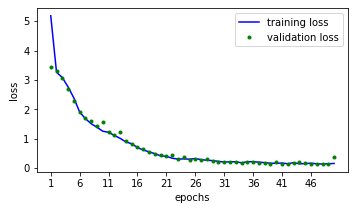
\includegraphics[width=.8\linewidth]{2DLossPool}  
    \caption[2DPool]{2D Avec Pooling}
    \end{subfigure}
    \begin{subfigure}{.5\textwidth}
    \centering
    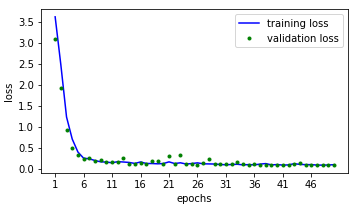
\includegraphics[width=.8\linewidth]{2DLossNoPool}  
    \caption[2DNoPool]{2D Sans Pooling}
    \end{subfigure}

    \centering
    \decoRule
    \caption[Loss en 2D]{Comparaison de la vitesse de decroissiance de la loss en 2D}
    \label{fig:2DLoss}
    \end{figure}

    COmme nous l'avons fait en 1D, Le modle sans max-pooling sera ulitlisee par la suite pour . Illustrons la correlation entre les predictions (de l'abcisse x, de l'ordonne y, et de la hauteur) et leurs labels repectifs (figure \ref{fig:Illustration2D}).
    \begin{figure}[!h]
    \begin{subfigure}{.33\textwidth}
    \centering
    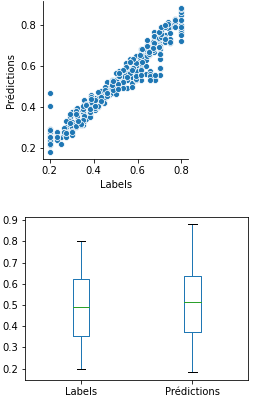
\includegraphics[width=.7\linewidth]{PositionX2D}  
    \caption[PosX2D]{Abcisse}
    \end{subfigure}
    \begin{subfigure}{.33\textwidth}
    \centering
    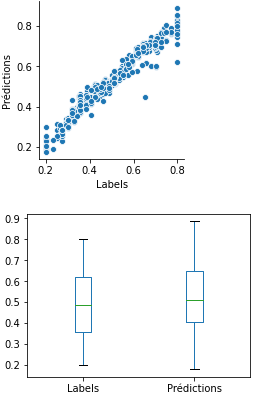
\includegraphics[width=.7\linewidth]{PositionY2D}  
    \caption[PosY2D]{Ordonee}
    \end{subfigure}
    \begin{subfigure}{.33\textwidth}
    \centering
    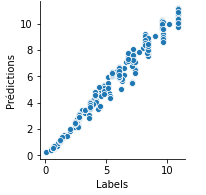
\includegraphics[width=.7\linewidth]{Hauteur2D}  
    \caption[H2D]{Hauteur}
    \end{subfigure}
    
     \centering
    \decoRule
    \caption[Illustration 2D]{Illustration de la correlation entre les labels et les predictions obtenues par le modele sans max-pooling en 2D. On peut observer que toutes les trois informations sont relativement bien correlee, d'ou le score R2 eleve (tableau \ref{tab:Tab2D}).}
    \label{fig:Illustration2D}
    \end{figure}
    
    Pour observer les meilleures et les pires predictions du modele, ils nous faut une mesure de la distance entre les predictions et les labels. On definit donc la norme ci-bas (en prenant soins de normaliser la hauteur). $$ \text{Norme} = \sqrt{\text{Abcisse}^2 + \text{Ordonee}^2 + \left( \frac{\text{Hauteur}}{10} \right)^2}$$
    
    \begin{figure}[!h]
    \begin{subfigure}{.5\textwidth}
    \centering
    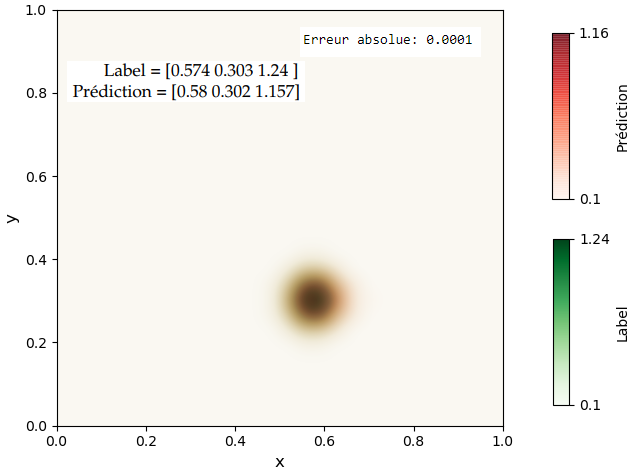
\includegraphics[width=.8\linewidth]{Meilleur2D1}  
    \caption[Meilleur2D1]{Label = [0.574 0.303 1.24 ] \\ Prediction = [0.58  0.302 1.157]}
    \end{subfigure}
    \begin{subfigure}{.5\textwidth}
    \centering
    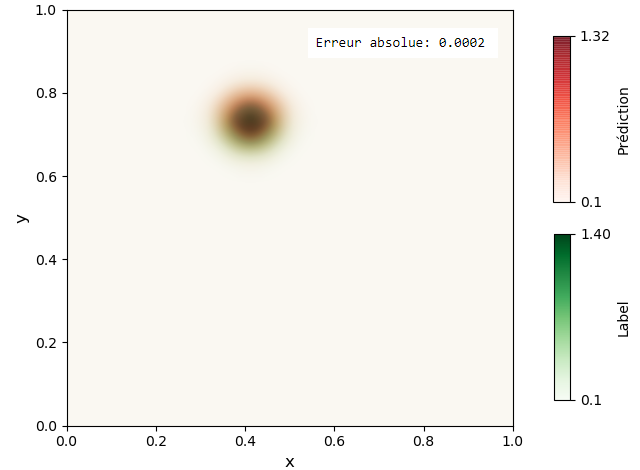
\includegraphics[width=.8\linewidth]{Meilleur2D2}  
    \caption[Meilleur2D2]{Label = [0.405 0.724 1.392]  \\  Prediction = [0.409 0.736 1.318]}
    \end{subfigure}
    
     \centering
    \decoRule
    \caption[Meilleur 2D]{Les meilleures predictions 2D. Ces images ont ete reconstruite a partir des  vecteurs "Labels" et "Prediction" issus de l'apprentissage. La premiere coordonne indique l'abcisse x du saut de densite, la deuxieme son ordonee y, et la troisieme sa hauteur. L'interpolation bicubique a ete utilise pour obtenir des images plus nettes.}
    \label{fig:Meilleur2D}
    \end{figure}

    \begin{figure}[H]
    \begin{subfigure}{.33\textwidth}
    \centering
    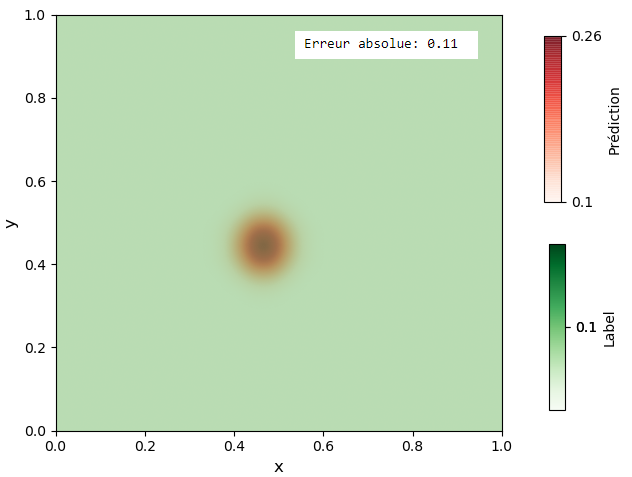
\includegraphics[width=1\linewidth]{Pire2D1}  
    \caption[Pire2D1]{Label = [0.2  0.65 0.1 ] \\ Prediction = [0.466 0.448 0.267]}
    \end{subfigure}
    \begin{subfigure}{.33\textwidth}
    \centering
    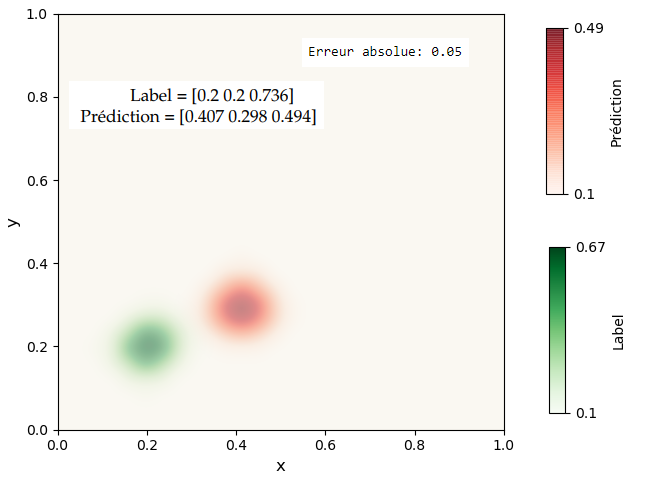
\includegraphics[width=1\linewidth]{Pire2D2}  
    \caption[Pire2D2]{Label = [0.2   0.2   0.736]  \\ Prediction = [0.407 0.298 0.494]}
    \end{subfigure}
    \begin{subfigure}{.33\textwidth}
    \centering
    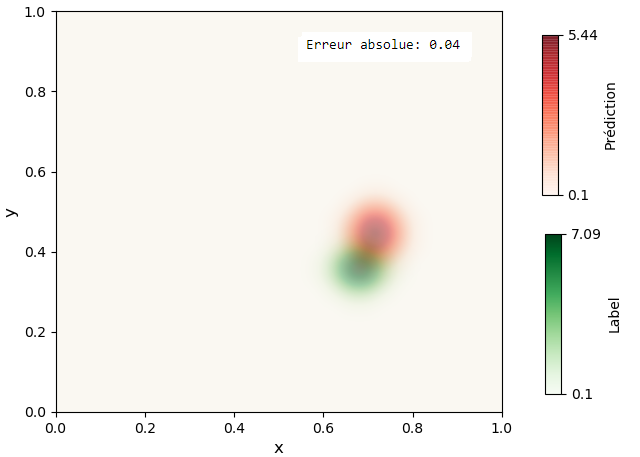
\includegraphics[width=1\linewidth]{Pire2D3}  
    \caption[Pire2D3]{Label = [0.674 0.358 7.096]  \\ Prediction = [0.712 0.449 5.462]}
    \end{subfigure}

     \centering
    \decoRule
    \caption[Pire2D]{Les pires prediction du modele 2D. Sans surprise la plus mauvaise des prediction s'obtient lorsque le crenau est absent (A). On remarque en general que les pires predictions sont faites lorsque le crenaus se situe tres proche de l'extremite (B).}
    \label{fig:Pire2D}
    \end{figure}
    
    En ce qui concerne la generalisation du modle a d'autres formes d'obstacles, je n'ai pas eu l'ocasion de comparer les modeles avec et sans max-Pooling. Le modele sans MaxPooling risque alors d'etre moins performant conformement a la theorie (voir paragraphe \ref{subsec:MaxPoling}). Sous Keras, le modele a prouver etre capable d'apprendre en continu, du moment que les entrees soient toutes normalisee et ayant la meme forme.

\subsection{Classification}
Durant le stage, il a fallu effectuer une classification mutilabel sur les donnes en 2D. QUi permet de placer l'obstacle dans une categorie definie a partir de la source. La classification petmet de detecter juste l;ordonne de l'obstacle. La structure des entrees est quasiment la meme que pour la regression, sauf qu'il manque les signaux sur la gauche (ou se trouve la source). En ce qui concerne les sorties, l'image ci-dessous decrit mieux leur structure:

\begin{figure}[!h] 
\centering
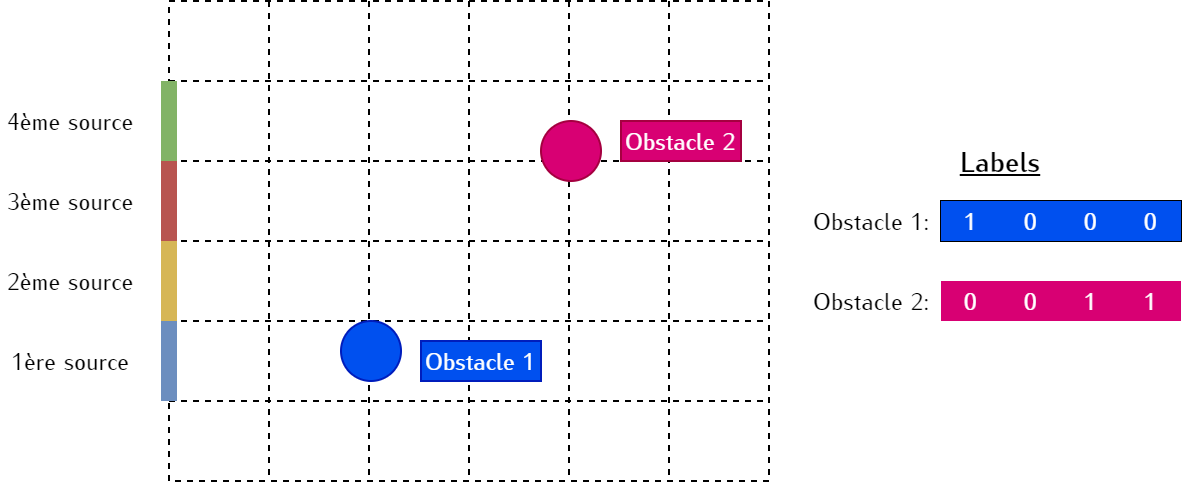
\includegraphics[width=.8\linewidth]{Classification} 
\decoRule
\caption[Classification]{Description des labels pour la classification multilabel en 2D. Un label est marque 1 si l'obstacle se touve dans le champ de la source correpondante}
\label{fig:Classification}
\end{figure}

Les donnnes utilisee pour la classification ont une shape differente des autre. On a moins d'iterations en temps (40 au lieu de 168) mais mais un maille beacoup plus fin (90x90 au lieu de 28x28). L'architecture du modle utilise ressemble celle de la regression. Une majeure difference est qu'on utilise une activation "sigmoid" a la place de l'activation "lineaire". On obtient donc en sortie des probabilites qu'il faut classer par categories. Le modele est entraine avec des hyper-parametres identiques a ceux utilisees durant les regression. Les resultats sont presentes a la table \ref{tab:Class}

\begin{table}[h!]
\caption{Resultats obtenus pour la classification en 2D. Le score severe favorise les predictions qui sont exactes au veritable sur tous les 4 colones . Le seuillage permet d'augmenter la precision des resultats en se fixant un nouveu seuil a partir duquel les interpreter les sorties du reseau de neurones. Le score de Binary Accuracy procure par keras est calcule avant seuillage.}
\label{tab:Class}
\centering
\begin{tabular}{l l l}
\toprule
\tabhead{Score} & \tabhead{Avec MaxPooling} & \tabhead{Sans MaxPooling} \\
\midrule
Binary accuracy & 75.00 \% & 98.86 \%\\
Score severe apres seillage & 27.27 \% & 95.45 \%\\
\bottomrule\\
\end{tabular}
\end{table}

\begin{figure}[!h]
\begin{subfigure}{.5\textwidth}
\centering
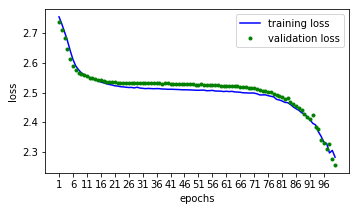
\includegraphics[width=.8\linewidth]{ClassPool}  
\caption[2DPool]{2D Avec Pooling}
\end{subfigure}
\begin{subfigure}{.5\textwidth}
\centering
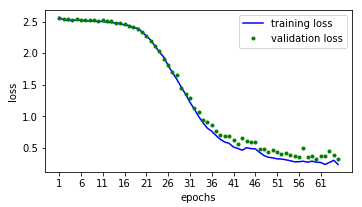
\includegraphics[width=.8\linewidth]{ClassNoPool}  
\caption[2DNoPool]{2D Sans Pooling}
\end{subfigure}

\centering
\decoRule
\caption[ClassLoss]{Comparaison de la vitesse de decroissiance de la loss (multilabel crossentropy) pour la classification en 2D}
\label{fig:ClassLoss}
\end{figure}


\begin{figure}[H] 
\centering
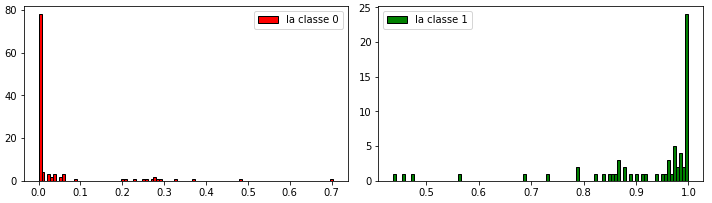
\includegraphics[width=.8\linewidth]{ClassFiabilite} 
\decoRule
\caption[ClassFiabilite]{Confiance du modele sans max-pooling en ses prediction. En rouge la classe 0 qui indique l'abscence du crenau devant la source; et en vert la classe 1. Cette figure indique que le modle se trompre rarement, ce qui confirme le resultat abtenu a la table \ref{tab:Class}.}
\label{fig:ClassFiabilite}
\end{figure}


Dans ce cas aussi, le modele sans Maxpooling seble meilleure (figures \ref{fig:ClassLoss} et \ref{fig:ClassFiabilite}). Cependant nous ne disposons pas d'axxez de donnes pour verifier celui qui se generalise mieux. Ceci etant une classifcation,  les meilleures prediction du meilleure modele sont exactement les labels attendus et les pires predictions ne varient que de peu (de 1) de leurs cibles. Il est interressnat de constater qu'il n'y a aucune prediction aberante, par exemple: un obstacle se trouve en face des sources 1 et 3 sans recontrer la source 2.

%----------------------------------------------------------------------------------------
